

%---------------------------------------------
%
%       START
%
%---------------------------------------------

\chapter[Missing data in living mammals]{Missing data in living mammals}
\label{chap:missing_mammals}

\bigskip
\medskip
\begin{center}

\noindent{\Large \bf Assessment of cladistic data availability for living mammals}
\footnote{A shorter version (2500 words) will be submitted under the same title to Biology Letters as an invited submission for a special issue on phylogenies with living and fossil species. This special issue is open to submission in December 2015. A pre-print is currently available at \url{http://dx.doi.org/10.1101/022970}.}
\footnote{T.G. and N.C. designed the experiments; T.G. ran the analysis and interpreted the results; T.G. and N.C. wrote the manuscripts.}
\footnote{\textit{Specific acknowledgements}: thanks to David Bapst, Graeme Lloyd, Nick Matzke and April Wright.}
\footnote{\textit{Data availability and reproducibility}: all data and analysis code is available on GitHub (\url{https://github.com/TGuillerme/Missing_living_mammals}).} \\
%} \\
% \medskip
% \noindent Key words: Total Evidence method, data structure, phylogenetic, fossil, topology\\
% \bigskip
% \noindent A shorter version (2500 words) will be submitted to Biology Letters as an invited submission for a special issue on phylogenies with living and fossil species. This special issue is open to submission in December 2015.\\

\end{center}
%---------------------------------------------
%
%       ABSTRACT
%
%---------------------------------------------


\begin{abstract}
Analyses of living and fossil taxa are crucial for understanding changes in biodiversity through time.
The Total Evidence method allows living and fossil taxa to be combined in phylogenies, by using molecular data for living taxa and morphological data for both living and fossil taxa.
With this method, substantial overlap of morphological data among living and fossil taxa is crucial for accurately inferring topology.
However, although molecular data for living species is widely available, scientists using and generating morphological data mainly focus on fossils.
Therefore, there is a gap in our knowledge of neontological morphological data even in well-studied groups such as mammals.

We investigated the amount of morphological (cladistic) data available for living mammals and how this data was phylogenetically distributed across orders.
22 of 28 mammalian orders have \textless 25\% species with available morphological data; this has implications for the accurate placement of fossil taxa, although the issue is less pronounced at higher taxonomic levels. 
In most orders, species with available data are randomly distributed across the phylogeny, which may reduce the impact of the problem.
We suggest that increased morphological data collection efforts for living taxa are needed to produce accurate Total Evidence phylogenies. 
\end{abstract}


\newpage

%---------------------------------------------
%
%       INTRODUCTION
%
%---------------------------------------------
\newpage 
\section{Introduction}
There is an increasing consensus among evolutionary biologists that studying both living and fossil taxa is essential for fully understanding macroevolutionary patterns and processes \citep{slaterunifying2013,fritzdiversity2013,Wood01032013}.
For example, including both living and fossil taxa in evolutionary studies can improve the accuracy of timing diversification events \citep[e.g.][]{ronquista2012}, our understanding of relationships among lineages \citep[e.g.][]{beckancient2014}, and our ability to infer biogeographical patterns through time \citep[e.g.][]{Meseguer01032015}.
To perform such analyses it is necessary to combine living and fossil taxa in phylogenetic trees.
One increasingly popular method, the Total Evidence method \citep{eernissetaxonomic1993,ronquista2012}, combines molecular data from living taxa and morphological data from both living and fossil taxa in a supermatrix \citep[e.g.][]{pyrondivergence2011,ronquista2012,schragocombining2013,slaterunifying2013,beckancient2014,Meseguer01032015}, producing a phylogeny with living and fossil taxa at the tips. 
These phylogenies can be dated using methods such as tip-dating \citep{ronquista2012,Wood01032013} and incorporated into macroevolutionary studies \citep[e.g.][]{ronquista2012,Wood01032013,slaterphylogenetic2013}.

A downside of the Total Evidence method is that it requires a lot of data.
One must collect molecular data for living taxa and morphological data for both living and fossil taxa; two types of data that require fairly different technical skills (e.g. molecular sequencing \textit{vs.} anatomical description).
Additionally, large chunks of this data can be difficult, or even impossible, to collect for every taxon present in the analysis.
For example, fossils very rarely have molecular data and incomplete fossil preservation (e.g. soft \textit{vs.} hard tissues) may restrict the amount of morphological data available \citep{sansomfossilization2013}.
Additionally, since the molecular phylogenetics revolution, it has become less common to collect morphological characters for living taxa when molecular data is available (e.g. in \citep{slaterphylogenetic2013}, only 13\% of the 169 living taxa have coded morphological data).
Unfortunately this missing data can lead to errors in phylogenetic inference; in fact, simulations show that the ability of the Total Evidence method to recover the correct phylogenetic topology decreases when there is a low overlap between morphological data in the living and fossil taxa \citep{GuillermeCooper}, regardless the overall amount of morphological data available for the fossils (or the amount of molecular data available for the living species).
The effect of missing data on topology is greatest when living taxa have few morphological data.
This is because (1) a fossil cannot branch in the correct clade if there is no overlapping morphological data in the clade; and (2) a fossil has a higher probability of branching within a clade with more morphological data available for living taxa, regardless of whether this is the correct clade or not \citep{GuillermeCooper}. 

The issues above highlight that it is crucial to have sufficient morphological data for living taxa in a clade before using a Total Evidence approach.
However, it is unclear how much morphological data for living taxa is actually available (i.e. already coded from museum specimens and deposited in phylogenetic matrices accessible online), and how this data is distributed across clades.
Intuitively, most people assume this kind of data has already been collected, but empirical data suggest otherwise (e.g. in \citep{ronquista2012,slaterphylogenetic2013,beckancient2014}.
To investigate this further, we assess the amount of available morphological data for living mammals to determine whether sufficient data exists to build reliable Total Evidence phylogenies in this group.
We collected cladistic data (i.e. discrete morphological characters used in phylogenetics) from 286 phylogenetic matrices available online and measured the proportion of cladistic data available for each mammalian order.
%Additionally, if the available data is randomly distributed across clades, the topological errors should be less extreme than if the data is biased towards particulars groups.
Additionally, because missing morphological data in living species can influence tree topology as described above, %NC: Might still need to fix this sentence. "Topological caveats above" was too unclear.
we determined whether the available cladistic data was phylogenetically overdispersed or clustered in the mammalian orders where data was missing. 
We find that available morphological data for living mammals is scarce but generally randomly distributed across phylogenies. 
We recommend that efforts be made to collect and share more cladistic data for living species to improve the accuracy of Total Evidence phylogenies.

% NC: If there are word count problems we can ditch the last two sentences.
%---------------------------------------------
%
%       METHODS
%
%---------------------------------------------
\section{Materials and Methods}
\subsection{Data collection and standardisation}
We downloaded all cladistic matrices containing any living and/or fossil mammal taxa from three major public databases (accessed 10th of June 2015): Morphobank (\url{http://www.morphobank.org/} \citep{morphobank}, Graeme Lloyd's website (\url{graemetlloyd.com/matrmamm.html} and Ross Mounce's GitHub repository (\url{https://github.com/rossmounce/cladistic-data}.
We also performed a systematic Google Scholar search (accessed 11th of June 2015) for matrices that were not uploaded to these databases. We downloaded available matrices containing fossil and/or living mammal taxa from the three data bases using the following list of keywords:

\texttt{Mammalia; Monotremata; Marsupialia; Placentalia; Macroscelidea; Afrosoricida; Tubulidentata; Hyracoidea; Proboscidea; Sirenia; Pilosa; Cingulata; Scandentia; Dermoptera; Primates; Lagomorpha; Rodentia; Erinaceomorpha; Soricomorpha; Cetacea; Artiodactyla; Cetartiodactyla; Chiroptera; Perissodactyla; Pholidota; Carnivora; Didelphimorphia; Paucituberculata; Microbiotheria; Dasyuromorphia; Peramelemorphia; Notoryctemorphia; Diprotodontia}.

Note that some matrices have been downloaded from more than one database but that it is not an issue since we are interested in the total number of unique living OTUs and that if some where present in more than one matrix, they still only counted as one single OTU.

\subsubsection*{Morphobank}
We used the keywords listed above in the search menu of the Morphobank repository (\texttt{http://www.morphobank.org/}) and downloaded the data associated with each project matching with the keywords.

\subsubsection*{Graeme Lloyd}
We downloaded all the matrices that were available with a direct download link in the mammal data section of Graeme Lloyd's website repository (\texttt{http://graemetlloyd.com/}).

\subsubsection*{Ross Mounce}
We downloaded every 601 matrix from Ross Mounce's GitHub repository (\texttt{https://github.com/rossmounce}) and then ran a shell script to select only the matrices that had any text element that match with one of the search terms.
To make the matrix selection more thorough, we ignored the keywords case as well as the latin suffix (\textit{ia}, \textit{ata}, \textit{ea}, and \textit{a}).

\subsubsection*{Google scholars}
To make sure we didn't miss any extra matrix that wasn't available on one of these repository, we ran a extra Google Scholar search. 
We downloaded the additional cladistic matrices from the 20 first search results matching with our selected keywords and with any of the 35 taxonomic levels (mammals Orders, Infraclasses and Class).
We used the following key words:

\texttt{\textit{order} ("morphology" OR "morphological" OR "cladistic") AND characters matrix paleontology phylogeny}

were \textit{order} was replaced by all the keywords listed above. For each 33 keywords, we selected the 20 first papers to match the Google search published since 2010 resulting in 660 papers.
Among these papers, not all contained relevant data (discrete morphological characters AND mammalian data).
We selected only the 20 first results per search term to avoid downloading articles that were to irrelevant. Among the 660 papers, only 50 contained a total of 425 extra living OTUs (Figure ~\ref{Supp_figure_google_searches}).
Also we decided to select only the articles published since 2010 because nearly every one of the recent published matrix contains both a fraction of morphological characters and OTUs from previous studies.
For example in primates the character \textit{p7} coded first by \cite{ross1998phylogenetic} is reused with the same living species in \cite{seiffert2003fossil}, \cite{marivaux2005anthropoid}, \cite{seiffert2005basal}, \cite{bloch2007new}, \cite{bloch2007new}, \cite{kay2008anatomy}, \cite{silcox2008biogeographic}, \cite{seiffert2009convergent}, \cite{tabuce2009anthropoid}, \cite{boyer2010astragalar}, \cite{seiffert2010fossil}, \cite{marivaux2013djebelemur} and \cite{ni2013oldest}.

\begin{figure}[!htbp]
\centering
    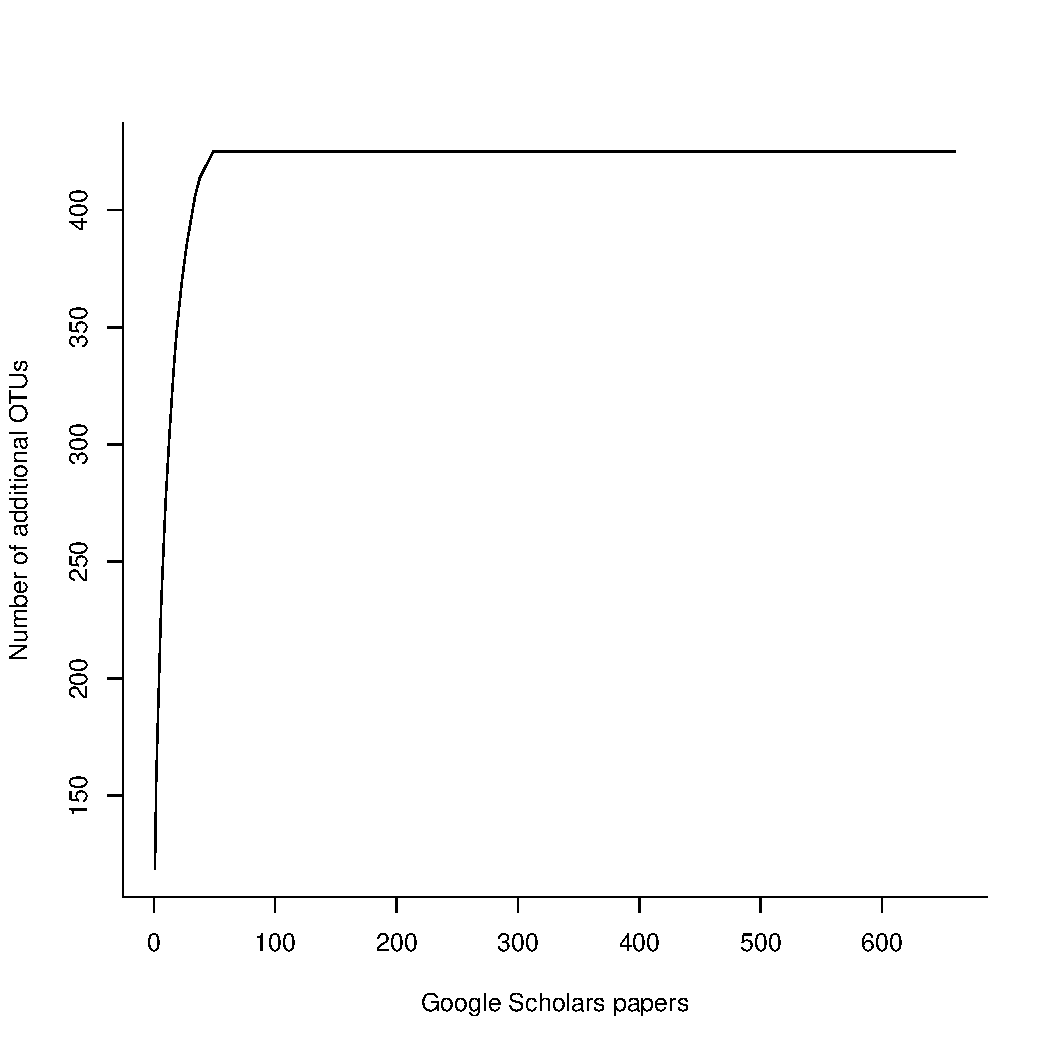
\includegraphics[width=1\textwidth]{Missing_mammals/Figures/Supp_figure_google_searches.pdf}
\caption[Google searches additional OTUs rarefaction curve.]{Google searches additional OTUs rarefaction curve. The x axis represent the number of google scholar matches (papers, books or abstracts) and the y axis represents the cumulative number of additional living OTUs per google scholar match.}
\label{Supp_figure_google_searches}
\end{figure}

We transformed all the non-nexus matrices (tnt, word, excel, jpeg) to nexus format manually.
In total, we downloaded 286 matrices containing a total of 11010 operational taxonomic units (OTUs) of which 5228 were unique.
In this study, we refer to OTUs rather than species since the entries in the downloaded matrices were not standardised and ranged from specific individual specimen names (i.e. the name of a collection item) to the family-level.
Where possible, we considered OTUs at their lowest valid taxonomic level (i.e. species) but some OTUs were only valid at a higher taxonomic level (e.g. genus or family).
Therefore for some orders, we sampled more genera than species (Table \ref{Table_morpho_taxa_proportion}.

To select the lowest valid taxonomic level for each OTU, we standardised their taxonomy by correcting species names so they matched standard taxonomic nomenclature (e.g., \textit{H. sapiens} was transformed to \textit{Homo sapiens}.
We designated as ``living'' all OTUs that were either present in the phylogeny of \citep{BinindaEmonds} or the taxonomy of \citep{wilson2005mammal}, and designated as ``fossil'' all OTUs that were present in the Paleobiology database (\url{https://paleobiodb.org/}.

For OTUs that did not appear in these three sources, we first decomposed the name (i.e. \textit{Homo sapiens} became \textit{Homo} and \textit{sapiens} and tried to match the first element with a higher taxonomic level (family, genus etc.).
Any OTUs that still had no matches in the sources above were designated as non-applicable (NA; see Figure \ref{Supp_figure_Taxonomic_algorithm}).

\begin{figure}[!htbp]
\centering
    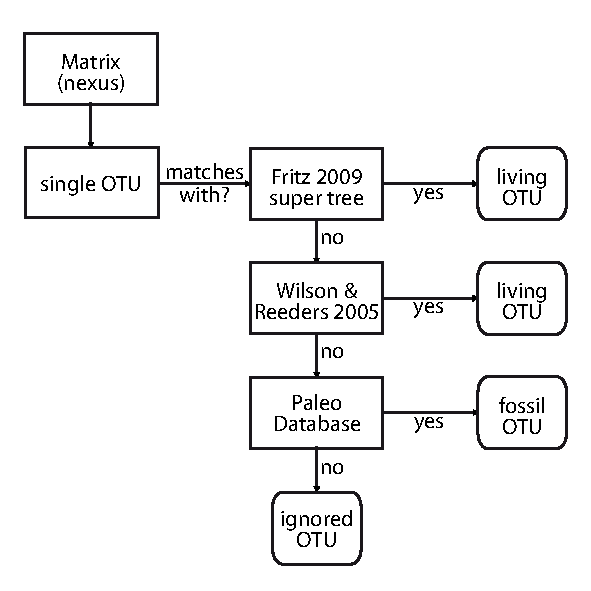
\includegraphics[width=1\textwidth]{Missing_mammals/Figures/Supp_figure_Taxonomic_algorithm.pdf}
\caption[Taxonomic matching algorithm used in this study.]{Taxonomic matching algorithm used in this study. For each matrix, each operational taxonomic units (OTU) is matched with the super tree from Bininda-Emonds 2007. If the OTU matches, then it is classified as living. Else it is matched with the Wilson \& Reeders 2005 taxonomy list. If the OTU matches, then it is classified as living. Else it is matched with the Paleo Database list of mammals. If the OTU matches, then it is classified as fossil. Else it is ignored.}
\label{Supp_figure_Taxonomic_algorithm}
\end{figure}

The number of characters in each matrix ranged from 6 to 4541.
Matrices with few characters are problematic when comparing available data among matrices because (1) they have less chance of having characters that overlap with those of other matrices \citep{wagner2000} and (2) they are more likely to contain a higher proportion of specific characters that are not-applicable across large clades (e.g. ``antler ramifications'' is a character that is only applicable to Cervidae not all mammals \citep{Brazeau2011}.
Therefore we selected only matrices containing \textgreater 100 characters for each OTU.
This threshold was chosen to correspond with the number of characters used in \citep{GuillermeCooper} and \citep{harrisonamong-character2014}.
Note that results of analyses with no character threshold are available in Supplementary Material. 
After removing all matrices with \textless 100 characters, we retained 1074 unique living mammal OTUs from 126 matrices for our analyses. % 1601 unique living OTUs for 286 matrices (no threshold)

\subsection{Data availability and distribution}
To assess the availability of cladistic data for each mammalian order, we calculated the percentage of OTUs with cladistic data at three different taxonomic levels: family, genus and species.
%We used these different taxonomic levels because some clades are well covered at the family- or genus-level, but poorly covered at the species-level. % NC: Probably obvious?
We consider orders with \textless 25\% of living taxa with cladistic data as having poor data coverage (``low'' coverage), and orders with \textgreater 75\% of living taxa with cladistic data as having good data coverage (hereafter ``high'' coverage). 

For orders with \textless 100\% cladistic data coverage at any taxonomic level, we investigated whether the available cladistic data was (i) randomly distributed, (ii) overdispersed or (iii) clustered, with respect to phylogeny, using two metrics from community phylogenetics: the Nearest Taxon Index (NTI; \citep{webb2002phylogenies} and the Net Relatedness Index (NRI; \citep{webb2002phylogenies}. 
NTI is most sensitive to clustering or overdispersion near the tips, whereas NRI is more sensitive to clustering or overdispersion across the whole phylogeny \citep{Cooper2008}. 
Both metrics were calculated using the \texttt{picante} package in R \citep{picante,R}.

NTI \citep{webb2002phylogenies} is based on mean nearest neighbour distance (MNND) and is calculated as follows:
  \begin{equation}
    NTI=-\left(\frac{\overline{MNND}_{obs}-\overline{MNND}_{n}}{\sigma(MNND_{n})}\right)
  \end{equation}
where $\overline{MNND}_{obs}$ is the observed mean distance between each of $n$ taxa with cladistic data and its nearest neighbour with cladistic data in the phylogeny, 
$\overline{MNND}_{n}$ is the mean of 1000 mean MNND between $n$ randomly drawn taxa, and $\sigma(MNND_{n})$ is the standard deviation of these 1000 random MNND values.
NRI is similar but is based on mean phylogenetic distance (MPD) as follows:
  \begin{equation}
    NRI=-\left(\frac{\overline{MPD}_{obs}-\overline{MPD}_{n}}{\sigma(MPD_{n})}\right)
  \end{equation}
where $\overline{MPD}_{obs}$ is the observed mean phylogenetic distance of the tree containing only the $n$ taxa with cladistic data, $\overline{MPD}_{n}$ is the expected random MPD for $n$ taxa estimated by calculating the MPD from $n$ taxa randomly drawn from the phylogeny and repeated 1000 times, and $\sigma(MPD_{n})$ is the standard deviation of the 1000 random MPD values. % NC: This can be shortened a bit but it's only gonna save you 50 words max.
Negative NTI and NRI values show that the focal taxa are more overdispersed across the phylogeny than expected by chance, and positive values reflect significant clustering.

We calculated NTI and NRI values for each mammalian order separately, at each different taxonomic level. 
For each analysis our focal taxa were those with available cladistic data at that taxonomic level and the phylogeny was the phylogeny of the order pruned from \citep{BinindaEmonds}.

%---------------------------------------------
%
%       RESULTS
%
%---------------------------------------------

\section{Results}
Across the 126 cladistic matrices we extracted, 22 out of 28 mammalian orders have low coverage (\textless 25\% of species with cladistic data) and six have high coverage (\textgreater 75\% of species with cladistic data) at the species-level.
At the genus-level, three orders have low coverage and 12 have high coverage, and at the family-level, no orders have low coverage and 23 have high coverage (Table \ref{Table_results}).

% latex table generated in R 3.2.0 by xtable 1.7-4 package
% Sun Jun 21 15:26:40 2015
\begin{longtable}{lL{1.8cm}C{2cm}lcc}
\caption{Number of taxa with available cladistic data for mammalian orders at three taxonomic levels. The left vertical bar represents ``low'' coverage (\textless 25\%); the right vertical bar represents ``high'' coverage (\textgreater 75\%). A negative Net Relatedness Index (NRI) and Nearest Taxon Index (NTI) shows more phylogeneticaly dispersed taxa than expected by chance; a positive value shows more phylogeneticaly clustered taxa than expected by chance. Significant NRI or NTI values are highlighted in bold. One star (*) signifies a p-value between 0.05 and 0.005; two starts between 0.005 and 0.0005 and three stars \textless 0.0005.} \\ 
  \hline
Order & Taxonomic level & Proportion of taxa & Coverage & NRI & NTI \\ 
  \hline
Afrosoricida & family & 2/2 & 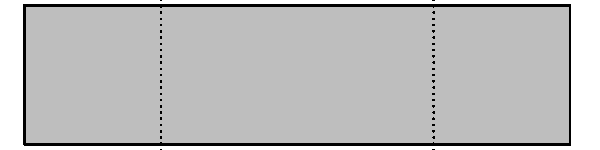
\includegraphics[width=0.20\linewidth, height=0.05\linewidth]{Missing_mammals/Table_figures/bar1.pdf} &   &   \\ 
  Afrosoricida & genus & 17/17 & 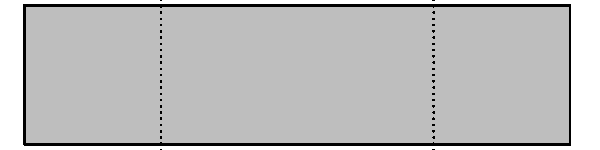
\includegraphics[width=0.20\linewidth, height=0.05\linewidth]{Missing_mammals/Table_figures/bar2.pdf} &   &   \\ 
  \textbf{Afrosoricida} & \textbf{species} & \textbf{23/42} & 
\includegraphics[width=0.20\linewidth, height=0.05\linewidth]{Missing_mammals/Table_figures/bar3.pdf} & \textbf{1.89*} & 1.19 \\ 
  Carnivora & family & 11/15 & 
\includegraphics[width=0.20\linewidth, height=0.05\linewidth]{Missing_mammals/Table_figures/bar4.pdf} & 0.43 & 1.68 \\ 
  \textbf{Carnivora} & \textbf{genus} & \textbf{30/125} & 
\includegraphics[width=0.20\linewidth, height=0.05\linewidth]{Missing_mammals/Table_figures/bar5.pdf} & \textbf{4.14**} & \textbf{1.81*} \\ 
  \textbf{Carnivora} & \textbf{species} & \textbf{42/283} & 
\includegraphics[width=0.20\linewidth, height=0.05\linewidth]{Missing_mammals/Table_figures/bar6.pdf} & \textbf{18.64**} & \textbf{3.02**} \\ 
  Cetartiodactyla & family & 21/21 & 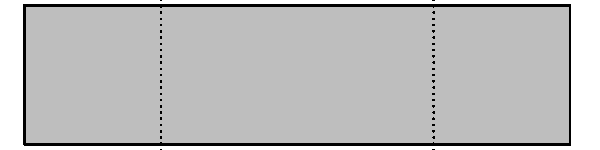
\includegraphics[width=0.20\linewidth, height=0.05\linewidth]{Missing_mammals/Table_figures/bar7.pdf} &   &   \\ 
  \textbf{Cetartiodactyla} & \textbf{genus} & \textbf{77/128} & 
\includegraphics[width=0.20\linewidth, height=0.05\linewidth]{Missing_mammals/Table_figures/bar8.pdf} & 0.87 & \textbf{1.77*} \\ 
  \textbf{Cetartiodactyla} & \textbf{species} & \textbf{129/310} & 
\includegraphics[width=0.20\linewidth, height=0.05\linewidth]{Missing_mammals/Table_figures/bar9.pdf} & \textbf{2.72*} & 0.04 \\ 
  Chiroptera & family & 13/18 & 
\includegraphics[width=0.20\linewidth, height=0.05\linewidth]{Missing_mammals/Table_figures/bar10.pdf} & 0.55 & 0.63 \\ 
  \textbf{Chiroptera} & \textbf{genus} & \textbf{85/202} & 
\includegraphics[width=0.20\linewidth, height=0.05\linewidth]{Missing_mammals/Table_figures/bar11.pdf} & \textbf{16.91**} & \textbf{2.85**} \\ 
  \textbf{Chiroptera} & \textbf{species} & \textbf{165/1053} & 
\includegraphics[width=0.20\linewidth, height=0.05\linewidth]{Missing_mammals/Table_figures/bar12.pdf} & \textbf{14.55**} & \textbf{3.44**} \\ 
  Cingulata & family & 1/1 & 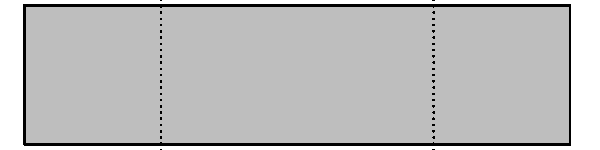
\includegraphics[width=0.20\linewidth, height=0.05\linewidth]{Missing_mammals/Table_figures/bar13.pdf} &   &   \\ 
  Cingulata & genus & 8/9 & 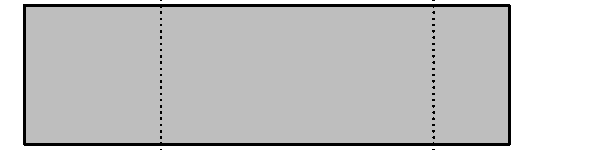
\includegraphics[width=0.20\linewidth, height=0.05\linewidth]{Missing_mammals/Table_figures/bar14.pdf} & 1.49 & -1.63 \\ 
  Cingulata & species & 6/29 & 
\includegraphics[width=0.20\linewidth, height=0.05\linewidth]{Missing_mammals/Table_figures/bar15.pdf} & 1.43 & 0.36 \\ 
  Dasyuromorphia & family & 2/2 & 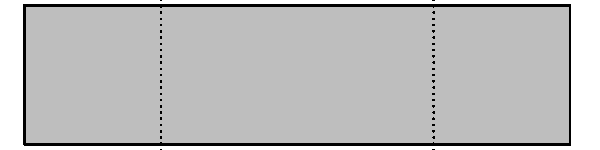
\includegraphics[width=0.20\linewidth, height=0.05\linewidth]{Missing_mammals/Table_figures/bar16.pdf} &   &   \\ 
  Dasyuromorphia & genus & 7/22 & 
\includegraphics[width=0.20\linewidth, height=0.05\linewidth]{Missing_mammals/Table_figures/bar17.pdf} & -1 & -1.45 \\ 
  Dasyuromorphia & species & 8/64 & 
\includegraphics[width=0.20\linewidth, height=0.05\linewidth]{Missing_mammals/Table_figures/bar18.pdf} & -1.15 & -0.62 \\ 
  Dermoptera & family & 1/1 & 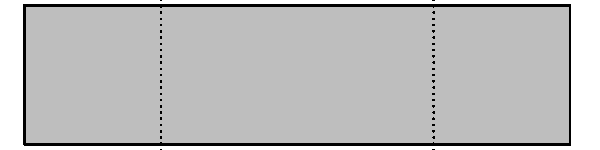
\includegraphics[width=0.20\linewidth, height=0.05\linewidth]{Missing_mammals/Table_figures/bar19.pdf} &   &   \\ 
  Dermoptera & genus & 1/2 & 
\includegraphics[width=0.20\linewidth, height=0.05\linewidth]{Missing_mammals/Table_figures/bar20.pdf} &   &   \\ 
  Dermoptera & species & 1/2 & 
\includegraphics[width=0.20\linewidth, height=0.05\linewidth]{Missing_mammals/Table_figures/bar21.pdf} &   &   \\ 
  Didelphimorphia & family & 1/1 & 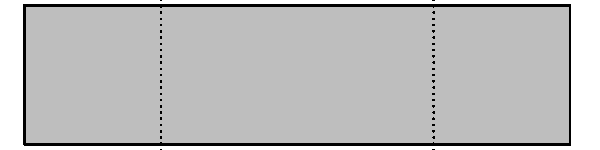
\includegraphics[width=0.20\linewidth, height=0.05\linewidth]{Missing_mammals/Table_figures/bar22.pdf} &   &   \\ 
  Didelphimorphia & genus & 16/16 & 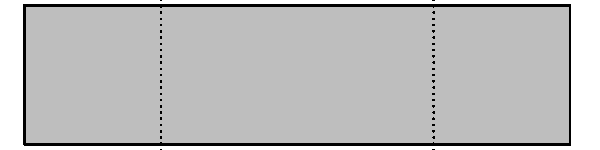
\includegraphics[width=0.20\linewidth, height=0.05\linewidth]{Missing_mammals/Table_figures/bar23.pdf} &   &   \\ 
  Didelphimorphia & species & 40/84 & 
\includegraphics[width=0.20\linewidth, height=0.05\linewidth]{Missing_mammals/Table_figures/bar24.pdf} & -0.94 & 0.36 \\ 
  Diprotodontia & family & 9/11 & 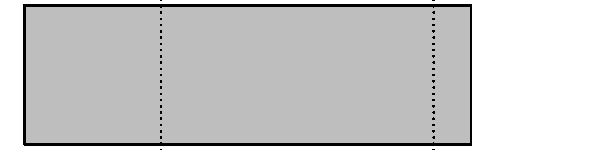
\includegraphics[width=0.20\linewidth, height=0.05\linewidth]{Missing_mammals/Table_figures/bar25.pdf} & -0.8 & 0.56 \\ 
  Diprotodontia & genus & 20/38 & 
\includegraphics[width=0.20\linewidth, height=0.05\linewidth]{Missing_mammals/Table_figures/bar26.pdf} & -1.36 & -0.73 \\ 
  Diprotodontia & species & 16/126 & 
\includegraphics[width=0.20\linewidth, height=0.05\linewidth]{Missing_mammals/Table_figures/bar27.pdf} & -2.29 & -1.55 \\ 
  Erinaceomorpha & family & 1/1 & 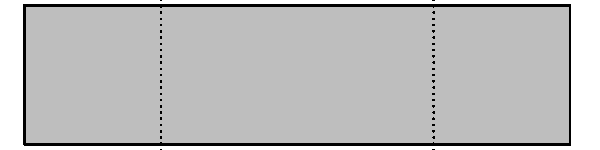
\includegraphics[width=0.20\linewidth, height=0.05\linewidth]{Missing_mammals/Table_figures/bar28.pdf} &   &   \\ 
  Erinaceomorpha & genus & 10/10 & 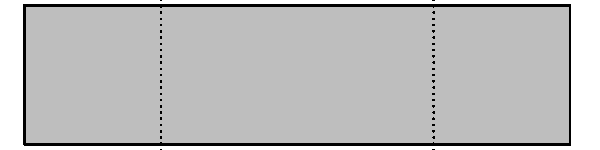
\includegraphics[width=0.20\linewidth, height=0.05\linewidth]{Missing_mammals/Table_figures/bar29.pdf} &   &   \\ 
  Erinaceomorpha & species & 21/22 & 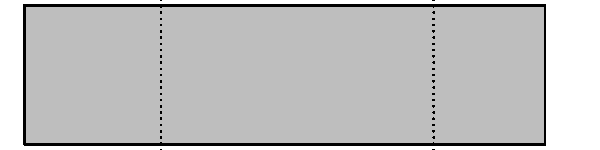
\includegraphics[width=0.20\linewidth, height=0.05\linewidth]{Missing_mammals/Table_figures/bar30.pdf} & -1.1 & -0.3 \\ 
  Hyracoidea & family & 1/1 & 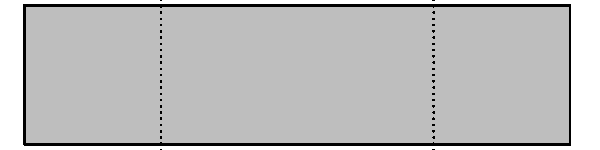
\includegraphics[width=0.20\linewidth, height=0.05\linewidth]{Missing_mammals/Table_figures/bar31.pdf} &   &   \\ 
  Hyracoidea & genus & 1/3 & 
\includegraphics[width=0.20\linewidth, height=0.05\linewidth]{Missing_mammals/Table_figures/bar32.pdf} &   &   \\ 
  Hyracoidea & species & 1/4 & 
\includegraphics[width=0.20\linewidth, height=0.05\linewidth]{Missing_mammals/Table_figures/bar33.pdf} &   &   \\ 
  Lagomorpha & family & 1/2 & 
\includegraphics[width=0.20\linewidth, height=0.05\linewidth]{Missing_mammals/Table_figures/bar34.pdf} &   &   \\ 
  Lagomorpha & genus & 1/12 & 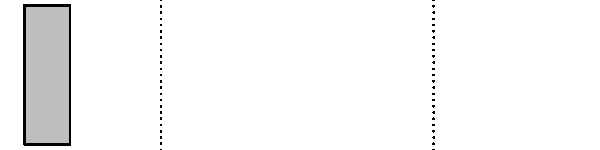
\includegraphics[width=0.20\linewidth, height=0.05\linewidth]{Missing_mammals/Table_figures/bar35.pdf} &   &   \\ 
  Lagomorpha & species & 1/86 & 
\includegraphics[width=0.20\linewidth, height=0.05\linewidth]{Missing_mammals/Table_figures/bar36.pdf} &   &   \\ 
  Macroscelidea & family & 1/1 & 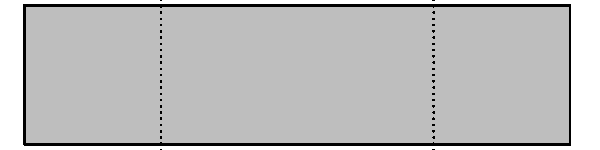
\includegraphics[width=0.20\linewidth, height=0.05\linewidth]{Missing_mammals/Table_figures/bar37.pdf} &   &   \\ 
  Macroscelidea & genus & 4/4 & 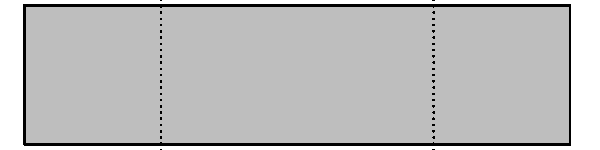
\includegraphics[width=0.20\linewidth, height=0.05\linewidth]{Missing_mammals/Table_figures/bar38.pdf} &   &   \\ 
  Macroscelidea & species & 5/15 & 
\includegraphics[width=0.20\linewidth, height=0.05\linewidth]{Missing_mammals/Table_figures/bar39.pdf} & -0.98 & -1.38 \\ 
  Microbiotheria & family & 1/1 & 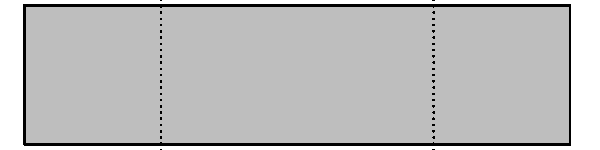
\includegraphics[width=0.20\linewidth, height=0.05\linewidth]{Missing_mammals/Table_figures/bar40.pdf} &   &   \\ 
  Microbiotheria & genus & 1/1 & 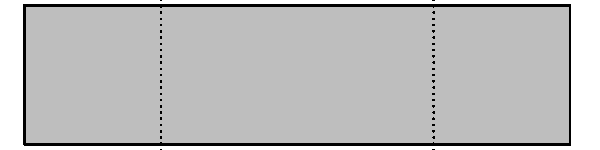
\includegraphics[width=0.20\linewidth, height=0.05\linewidth]{Missing_mammals/Table_figures/bar41.pdf} &   &   \\ 
  Microbiotheria & species & 1/1 & 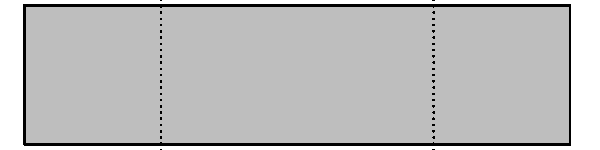
\includegraphics[width=0.20\linewidth, height=0.05\linewidth]{Missing_mammals/Table_figures/bar42.pdf} &   &   \\ 
  Monotremata & family & 2/2 & 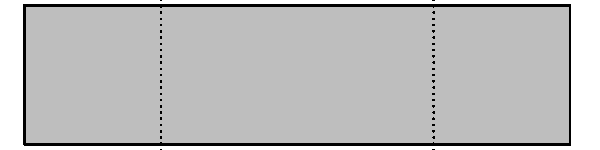
\includegraphics[width=0.20\linewidth, height=0.05\linewidth]{Missing_mammals/Table_figures/bar43.pdf} &   &   \\ 
  Monotremata & genus & 2/3 & 
\includegraphics[width=0.20\linewidth, height=0.05\linewidth]{Missing_mammals/Table_figures/bar44.pdf} & -0.71 & -0.71 \\ 
  Monotremata & species & 2/4 & 
\includegraphics[width=0.20\linewidth, height=0.05\linewidth]{Missing_mammals/Table_figures/bar45.pdf} & -1.01 & -1.03 \\ 
  Notoryctemorphia & family & 1/1 & 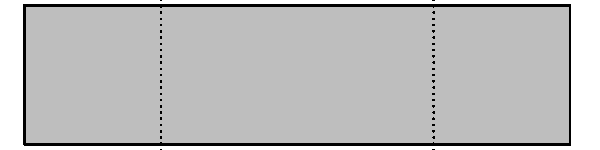
\includegraphics[width=0.20\linewidth, height=0.05\linewidth]{Missing_mammals/Table_figures/bar46.pdf} &   &   \\ 
  Notoryctemorphia & genus & 1/1 & 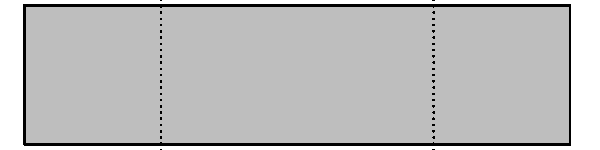
\includegraphics[width=0.20\linewidth, height=0.05\linewidth]{Missing_mammals/Table_figures/bar47.pdf} &   &   \\ 
  Notoryctemorphia & species & 0/2 & 
\includegraphics[width=0.20\linewidth, height=0.05\linewidth]{Missing_mammals/Table_figures/bar48.pdf} &   &   \\ 
  Paucituberculata & family & 1/1 & \includegraphics[width=0.20\linewidth, height=0.05\linewidth]{Missing_mammals/Table_figures/bar49.pdf} &   &   \\ 
  Paucituberculata & genus & 2/3 & \includegraphics[width=0.20\linewidth, height=0.05\linewidth]{Missing_mammals/Table_figures/bar50.pdf} & 0 & 0 \\ 
  Paucituberculata & species & 2/5 & \includegraphics[width=0.20\linewidth, height=0.05\linewidth]{Missing_mammals/Table_figures/bar51.pdf} & -0.64 & -0.65 \\ 
  Peramelemorphia & family & 2/2 & \includegraphics[width=0.20\linewidth, height=0.05\linewidth]{Missing_mammals/Table_figures/bar52.pdf} &   &   \\ 
  Peramelemorphia & genus & 7/7 & \includegraphics[width=0.20\linewidth, height=0.05\linewidth]{Missing_mammals/Table_figures/bar53.pdf} &   &   \\ 
  Peramelemorphia & species & 16/18 & \includegraphics[width=0.20\linewidth, height=0.05\linewidth]{Missing_mammals/Table_figures/bar54.pdf} & -0.09 & 1 \\ 
  Perissodactyla & family & 3/3 & \includegraphics[width=0.20\linewidth, height=0.05\linewidth]{Missing_mammals/Table_figures/bar55.pdf} &   &   \\ 
  Perissodactyla & genus & 6/6 & \includegraphics[width=0.20\linewidth, height=0.05\linewidth]{Missing_mammals/Table_figures/bar56.pdf} &   &   \\ 
  Perissodactyla & species & 7/16 & \includegraphics[width=0.20\linewidth, height=0.05\linewidth]{Missing_mammals/Table_figures/bar57.pdf} & 0.62 & -2.5 \\ 
  Pholidota & family & 1/1 & \includegraphics[width=0.20\linewidth, height=0.05\linewidth]{Missing_mammals/Table_figures/bar58.pdf} &   &   \\ 
  Pholidota & genus & 1/1 & \includegraphics[width=0.20\linewidth, height=0.05\linewidth]{Missing_mammals/Table_figures/bar59.pdf} &   &   \\ 
  \textbf{Pholidota} & \textbf{species} & \textbf{3/8} & \includegraphics[width=0.20\linewidth, height=0.05\linewidth]{Missing_mammals/Table_figures/bar60.pdf} & \textbf{2.64*} & \textbf{2.23*} \\ 
  Pilosa & family & 3/5 & \includegraphics[width=0.20\linewidth, height=0.05\linewidth]{Missing_mammals/Table_figures/bar61.pdf} & 0.94 & 0.93 \\ 
  Pilosa & genus & 3/5 & \includegraphics[width=0.20\linewidth, height=0.05\linewidth]{Missing_mammals/Table_figures/bar62.pdf} & -0.36 & -0.31 \\ 
  Pilosa & species & 3/29 & \includegraphics[width=0.20\linewidth, height=0.05\linewidth]{Missing_mammals/Table_figures/bar63.pdf} & 0.33 & 0.79 \\ 
  Primates & family & 15/15 & \includegraphics[width=0.20\linewidth, height=0.05\linewidth]{Missing_mammals/Table_figures/bar64.pdf} &   &   \\ 
  Primates & genus & 48/68 & \includegraphics[width=0.20\linewidth, height=0.05\linewidth]{Missing_mammals/Table_figures/bar65.pdf} & -0.41 & -1.4 \\ 
  Primates & species & 56/351 & \includegraphics[width=0.20\linewidth, height=0.05\linewidth]{Missing_mammals/Table_figures/bar66.pdf} & -1.6 & -2.04 \\ 
  Proboscidea & family & 1/1 & \includegraphics[width=0.20\linewidth, height=0.05\linewidth]{Missing_mammals/Table_figures/bar67.pdf} &   &   \\ 
  Proboscidea & genus & 1/2 & \includegraphics[width=0.20\linewidth, height=0.05\linewidth]{Missing_mammals/Table_figures/bar68.pdf} &   &   \\ 
  Proboscidea & species & 1/3 & \includegraphics[width=0.20\linewidth, height=0.05\linewidth]{Missing_mammals/Table_figures/bar69.pdf} &   &   \\ 
  Rodentia & family & 11/32 & \includegraphics[width=0.20\linewidth, height=0.05\linewidth]{Missing_mammals/Table_figures/bar70.pdf} & -0.46 & -1.91 \\ 
  Rodentia & genus & 21/450 & \includegraphics[width=0.20\linewidth, height=0.05\linewidth]{Missing_mammals/Table_figures/bar71.pdf} & -2.11 & 0.3 \\ 
  Rodentia & species & 15/2094 & \includegraphics[width=0.20\linewidth, height=0.05\linewidth]{Missing_mammals/Table_figures/bar72.pdf} & -1.65 & -2.55 \\ 
  Scandentia & family & 2/2 & \includegraphics[width=0.20\linewidth, height=0.05\linewidth]{Missing_mammals/Table_figures/bar73.pdf} &   &   \\ 
  Scandentia & genus & 2/5 & \includegraphics[width=0.20\linewidth, height=0.05\linewidth]{Missing_mammals/Table_figures/bar74.pdf} & -0.77 & -0.76 \\ 
  Scandentia & species & 2/20 & \includegraphics[width=0.20\linewidth, height=0.05\linewidth]{Missing_mammals/Table_figures/bar75.pdf} & -1.79 & -1.99 \\ 
  Sirenia & family & 2/2 & \includegraphics[width=0.20\linewidth, height=0.05\linewidth]{Missing_mammals/Table_figures/bar76.pdf} &   &   \\ 
  Sirenia & genus & 2/2 & \includegraphics[width=0.20\linewidth, height=0.05\linewidth]{Missing_mammals/Table_figures/bar77.pdf} &   &   \\ 
  Sirenia & species & 4/4 & \includegraphics[width=0.20\linewidth, height=0.05\linewidth]{Missing_mammals/Table_figures/bar78.pdf} &   &   \\ 
  Soricomorpha & family & 3/4 & \includegraphics[width=0.20\linewidth, height=0.05\linewidth]{Missing_mammals/Table_figures/bar79.pdf} & -0.93 & -0.92 \\ 
  \textbf{Soricomorpha} & \textbf{genus} & \textbf{19/43} & \includegraphics[width=0.20\linewidth, height=0.05\linewidth]{Missing_mammals/Table_figures/bar80.pdf} & \textbf{6.98**} & \textbf{2.49*} \\ 
  \textbf{Soricomorpha} & \textbf{species} & \textbf{19/392} & \includegraphics[width=0.20\linewidth, height=0.05\linewidth]{Missing_mammals/Table_figures/bar81.pdf} & \textbf{13.19**} & \textbf{3.89**} \\ 
  Tubulidentata & family & 1/1 & \includegraphics[width=0.20\linewidth, height=0.05\linewidth]{Missing_mammals/Table_figures/bar82.pdf} &   &   \\ 
  Tubulidentata & genus & 1/1 & \includegraphics[width=0.20\linewidth, height=0.05\linewidth]{Missing_mammals/Table_figures/bar83.pdf} &   &   \\ 
  Tubulidentata & species & 1/1 & \includegraphics[width=0.20\linewidth, height=0.05\linewidth]{Missing_mammals/Table_figures/bar84.pdf} &   &   \\ 
   \hline
\hline
\label{Table_results}
\end{longtable}


Among the mammalian orders containing OTUs with no available cladistic data, only six orders had significantly clustered data (Carnivora, Cetartiodactyla, Chiroptera and Soricomorpha at both species- and genus-level and Afrosoricida and Pholidota at the species-level only) and no order had significantly overdispersed data at any taxonomic level (Table~\ref{Table_results}).

Two contrasting results are shown in Figure \ref{Figure_example_coverage} with randomly distributed OTUs with cladistic data in Primates (Figure \ref{Figure_example_coverage}A) and phylogenetically clustered OTUs with cladistic data in Carnivora (mainly Canidae; Figure \ref{Figure_example_coverage}B).

\begin{figure}[!htbp]
\centering
    \includegraphics[width=1\textwidth]{Missing_mammals/Figures/example_coverage.pdf}
\caption[Phylogenetic distribution of species with available cladistic data across Primates and Carnivora]{Phylogenetic distribution of species with available cladistic data across two mammalian orders (A: Primates; B: Carnivora).
Edges are colored in grey when no cladistic data is available for a species and in blue when data is available.}
\label{Figure_example_coverage}
\end{figure}

%---------------------------------------------
%
%       DISCUSSION
%
%---------------------------------------------

\section{Discussion}
Our results show that although phylogenetic relationships among living mammals are well-resolved \citep[e.g.][]{BinindaEmonds,meredithimpacts2011} , most of the data used to build these phylogenies is molecular, and very little cladistic data is available for living mammals compared to fossil mammals \citep[e.g.][]{O'Leary08022013,ni2013oldest}.
This has implications for building Total Evidence phylogenies containing both living and fossil mammals, as without sufficient cladistic data for living species, fossil placements in these trees are very uncertain \citep{GuillermeCooper}.
Cladistic data coverage in living mammals varies across taxonomic levels and in its phylogenetic distribution.
Higher taxonomic levels are always better sampled than lower ones and within these taxonomic levels, the available data is mostly randomly distributed across the phylogeny, apart from in six orders).

The number of living mammalian taxa with no available cladistic data was surprisingly high at the species-level: only six out of 28 orders have a high coverage of taxa with available cladistic data (and two of the 28 orders are monospecific!).
This high coverage threshold of 75\% of taxa with available cladistic data represents the minimum amount of data required before missing data has a significant effect on the topology of Total Evidence trees \citep{GuillermeCooper}.
Beyond this threshold, there is considerable displacement of wildcard taxa (\textit{sensu} \citep{kearneyfragmentary2002} and decreases in clade conservation \citep{GuillermeCooper}.
Therefore we expect a high probability of topological artefacts for the placement of fossil taxa at the species-level in most mammalian orders.
However, data coverage seems to be less of an issue at higher taxonomic levels (i.e. genus- and family-level).
This point is important from a practical point of view because of the slight discrepancy between the neontological and palaeontological concept of species.
While neontological species are described using morphology, genetic distance, spatial distribution and even behaviour, palaeontological species can be based only on morphological, spatial and temporal data \citep[e.g.][]{ni2013oldest}.
Because of this, most palaeontological studies are using the genus as their smallest OTU \citep[e.g.][]{ni2013oldest,O'Leary08022013}.
Thus data availability at the genus-level in living mammals should be our primary concern when aiming to build phylogenies of living and fossil taxa.

When only a few species with cladistic data are available, the ideal scenario is for them to be phylogenetically overdispersed (i.e. that there is data for at least every sub-clade) to maximize the possibilities of a fossil branching from the right clade.
The second best scenario is that species with cladistic data are randomly distributed across the phylogeny. 
In this scenario we expect no special bias in the placement of the fossil \citep{GuillermeCooper}, it is therefore encouraging that for most orders, species with cladistic data were randomly distributed across the phylogeny of each order.
The worst case scenario for fossil placement is that species with cladistic data are phylogenetically clustered. 
In this situation we expect two major biases to occur: first, the fossil will not be able to branch within a clade containing no data, and second, the fossil will have a higher probability, at random, of branching within the clade containing most of the available data.
This means that fossils with uncertain phylogenetic affinities (\textit{incertae sedis} will have a higher probability of branching within the most sampled clade just by chance.
Our results suggest that this may be an issue, at the genus-level, in Carnivora, Cetartiodactyla, Chiroptera and Soricomorpha. 
For example, a Carnivora fossil will be unable to branch in the Herpestidae that has no species with cladistic data, and will also have more chance to branch, randomly, within the Canidae clade than any other clade in Carnivora (Figure \ref{Figure_example_coverage}B).
Thus, in Total Evidence trees, placements of some carnivoran fossils should considered with caution. 
% NC: Trying not to piss off GraHam - really it's weird stuff appearing in Carnivora that we are concerned by, not all Carnivora. TG: I think it's mainly Graham's work that focuses on canids.
In this study, we treated all cladistic matrices as equal in a similar way to molecular matrices. 
For example, if matrix A contained 100 characters for taxa X and Y, and matrix B contained 50 different characters for taxa X and Z, we assumed that both matrices can be combined in a supermatrix containing 150 independent characters for taxon X, 100 for taxon Y and 50 for taxon Z.
Unfortunately, cladistic data cannot always be treated in this way because some characters may overlap.
For example, if matrix A has a character coding for the shape of a particular morphological feature and matrix B has a character coding for the presence of this same morphological feature and a second character coding for its shape, then these three characters are non-independent compound characters \citep{Brazeau2011}.
However, in reasonably sized matrices (\textgreater 100 characters; \citep{GuillermeCooper,harrisonamong-character2014} it is more likely that a number of characters are consistently conserved among the different matrices and thus easily combinable.
For example, within the Primate cladistic literature, the character \textit{p7} - the size of the $4^{th}$ lower premolar paraconid - has been used consistently for \textgreater 15 years \citep[e.g.][]{ross1998phylogenetic,marivaux2005anthropoi,ni2013oldest} and can therefore be combined among the matrices.
A conservative approach to avoid compound characters would be to select only the most recent matrix for each group, but this would result in the loss of a lot of data.

Despite the absence of good cladistic data coverage for living mammals, the Total Evidence methods still seems to be the most promising way of combining living and fossil data for macroevolutionary analyses. 
Following the recommendations in \citep{GuillermeCooper}, we need to code cladistic characters for as many living species possible. 
Fortunately, data for living mammals is usually readily available in natural history collections, therefore, we propose that an increased effort be put into coding morphological characters from living species, possibly by engaging in collaborative data collection projects through web portals such as \textit{Morphobank} \citep{morphobank}.
% NC: Still feels like it needs one final sentence to round it all off. Many something like below, but less crappy:
Such an effort would be valuable not only to phylogeneticists, but also to any researcher focusing understanding macroevolutionary patterns and processes.%interested in the diversity of life on Earth.

%Biology letters various stuff

% \bibliographystyle{sysbio}
% \bibliography{References}

%\section{SOM}
%\newcommand{\beginsupplement}{%
%    \setcounter{table}{0}
%    \renewcommand{\thetable}{S\arabic{table}}%
%    \setcounter{figure}{0}
%    \renewcommand{\thefigure}{S\arabic{figure}}%
%}
%\beginsupplement
%
\noindent{\Large \bf Supplementary Material}

\begin{figure}[!htbp]
\centering
    \includegraphics[width=1\textwidth]{Missing_mammals/Supplementary/MissingDataFigure.pdf}
\caption{Example of topological errors due to missing morphological data in living taxa.
The phylogeny contains two clades, Aves and Mammalia, with molecular data (grey) for both but only morphological data (red) for Aves.
If a mammalian fossil species (with no molecular data) is added to the phylogeny, it will erroneously branch with the Aves instead of the Mammalia because no morphological data will overlap between the fossil mammals and the living ones.}
\label{Figure_missing_data_problem}
\end{figure}

\bigskip

\section{Data collection}
1- Data collection: key words, clade (ordinal) metacharacters, Google Search terms, Google Search protocol, Google Search rarefaction curve.

\subsection{Public repositories}
We downloaded available matrices containing fossil and/or living mammal taxa from the three following data bases using the following list of keywords:

\texttt{Mammalia; Monotremata; Marsupialia; Placentalia; Macroscelidea; Afrosoricida; Tubulidentata; Hyracoidea; Proboscidea; Sirenia; Pilosa; Cingulata; Scandentia; Dermoptera; Primates; Lagomorpha; Rodentia; Erinaceomorpha; Soricomorpha; Cetacea; Artiodactyla; Cetartiodactyla; Chiroptera; Perissodactyla; Pholidota; Carnivora; Didelphimorphia; Paucituberculata; Microbiotheria; Dasyuromorphia; Peramelemorphia; Notoryctemorphia; Diprotodontia}.

Details about each public repository specific search option is listed below. Note that some matrices have been downloaded from more than one database but that it is not an issue since we are interested in the total number of living OTUs and that if some where present in more than one matrix, they still only counted as a unique OTU.

\subsubsection{Morphobank}
We accessed the Morphobank repository (\texttt{http://www.morphobank.org/}) on the 5th of December 2014 and used the keywords listed above in the search menue. We downloaded the data associated with each project matching with the keyword.

\subsubsection{Graeme Lloyd}
We accessed Graeme Lloyd's website repository (\texttt{http://graemetlloyd.com/}) on the 5th of December 2014 and downloaded all the matrices that were available with a direct download link in the mammal data section of the website (\texttt{http://graemetlloyd.com/matrmamm.html}).

\subsubsection{Ross Mounce}
We accessed Ross Mounce's GitHub repository (\texttt{https://github.com/rossmounce}) on the 2nd of December 2014 and downloaded every 601 matrix. We then ran a shell script to select only the matrices that had any text element that match with one of the search terms. To make the matrix selection more thorough, we ignored the keywords case as well as the latin suffix (\textit{ia}, \textit{ata}, \textit{ea}, and \textit{a}).

\subsection{Google scholars}
To make sure we didn't miss any extra matrix that wasn't available on one of these repository, we ran a Google Scholar search on the 5th of January. 
We downloaded the additional cladistic matrices from the 20 first search results matching with our selected keywords and with any of the 35 taxonomic levels (mammals Orders, Infraclasses and Class).
We used the following key words:

\texttt{\textit{order} ("morphology" OR "morphological" OR "cladistic") AND characters matrix paleontology phylogeny}

were \textit{order} was replaced by all the keywords listed above. For each 33 keywords, we selected the 20 first papers to match the Google search published since 2010 resulting in 660 papers. Among these papers, not all contained relevant data (discrete morphological characters AND mammalian data). We selected only the 20 first results per search term to avoid downloading articles that were to irrelevant. Among the 660 papers, only 50 contained a total of 425 extra living OTUs (figure ~\ref{Supp_figure_google_searches}).
Also we decided to select only the articles published since 2010 because nearly every one of the recent published matrix contains both a fraction of morphological characters and OTUs from previous studies. For example in primates the character \textit{p7} coded first by \cite{ross1998phylogenetic} is reused with the same living species in \cite{seiffert2003fossil}, \cite{marivaux2005anthropoid}, \cite{seiffert2005basal}, \cite{bloch2007new}, \cite{bloch2007new}, \cite{kay2008anatomy}, \cite{silcox2008biogeographic}, \cite{seiffert2009convergent}, \cite{tabuce2009anthropoid}, \cite{boyer2010astragalar}, \cite{seiffert2010fossil}, \cite{marivaux2013djebelemur} and \cite{ni2013oldest}.

\begin{figure}[!htbp]
\centering
    \includegraphics[width=1\textwidth]{Missing_mammals/Supplementary/Supp_figure_google_searches.pdf}
\caption{Google searches additional OTUs rarefaction curve. The x axis represent the number of google scholar matches (papers, books or abstracts) and the y axis represents the cumulative number of additional living OTUs per google scholar match.}
\label{Supp_figure_google_searches}
\end{figure}

\subsection{Standardising the matrices}
We transformed all the non-nexus matrices (tnt, word, excel, jpeg) to nexus format manually. We then cleaned the nexus matrices by removing any extra information (trees, continuous characters, morphological characters description, molecular data) to end up with nexus matrices containing only the discrete morphological data. We then manually fixed the wrong bionomial names format (e.g. \textit{H. sapiens}) into the correct ones (e.g. \textit{Homo sapiens}) using the abbreviation list in the concerned publications. 

\subsection{Selecting the living OTUs}
Finally we applied a taxonomic matching algorithm to classify the OTUs as either living or fossil. The algorithm is matching every OTU name from every matrix with one of the following taxonomic references: the list of taxa from the Fritz \textit{et al.} supertree (2009) \cite{FritzTree}; the taxonomic list from the Wilson and Reeder's Mammals Species of the World (2005) \cite{wilson2005mammal} and the list of all the mammal fossil from the Paleobio Database (\texttt{http://paleobiodb.org/cgi-bin/bridge.pl?a=login}) accessed on the 13th of Janurary 2015. The OTUs that matched with one of the two first references were considered as living OTUs, the OTUs matching with the third reference were considered as fossil OTUs, finally, the OTUs matching with non of the references were discarded (figure ~\ref{Supp_figure_Taxonomic_algorithm}).

\begin{figure}[!htbp]
\centering
    \includegraphics[width=1\textwidth]{Missing_mammals/Supplementary/Supp_figure_Taxonomic_algorithm.pdf}
\caption{Taxonomic matching algorithm used in this study. For each matrix, each operational taxonomic units (OTU) is matched with the super tree from Fritz 2009. If the OTU matches, then it is classified as living. Else it is matched with the Wilson \& Reeders 2005 taxonomy list. If the OTU matches, then it is classified as living. Else it is matched with the Paleo Database list of mammals. If the OTU matches, then it is classified as fossil. Else it is ignored.}
\label{Supp_figure_Taxonomic_algorithm}
\end{figure}

%\bibliographystyle{vancouver}
%\bibliography{Supp_References}

\section{Supplementary results}
The following section contains supplementary results to the main body: the available data structure using the NTI and the PD metric; the proportion of available data and the data structure for all the matrices (including the matrices with less than 100 characters); and phylogenetical representation of the data availability per order (excluding Primates and Carnivora, present in the main body).

% latex table generated in R 3.2.0 by xtable 1.7-4 package
% Sat Jun 20 17:19:07 2015
\begin{longtable}{lL{1.8cm}C{2cm}lcc}
\caption{Number of taxa with available cladistic data for mammalian orders at three taxonomic levels (without any character threshold; results from the 286 matrices). The coverage represents the proportion of taxa with available morphological data. The left vertical bar represents 25\% of available data (``low'' coverage if \textless 25\%); The right vertical bar represents 75\% of available data (``high'' coverage if \textgreater 75\%). When the Net Relatedness Index (NRI) and the Nearest Taxon Index (NTI) are negative, taxa are more phylogenetically dispersed than expected by chance; when NRI or NTI are positive, taxa are more phylogenetically clustered by expected by chance. Significant NRI or NTI are highlighted in bold. One star (*) represents a p-value between 0.05 and 0.005; two starts between 0.005 and 0.0005 and three stars a p-value less than 0.0005.} \\ 
  \hline
Order & Taxonomic level & Proportion of taxa & Coverage & NRI & NTI \\ 
  \hline
Afrosoricida & family & 2/2 & \includegraphics[width=0.20\linewidth, height=0.05\linewidth]{Missing_mammals/Supplementary/Results_1c/Table_figures/bar1.pdf} &   &   \\ 
  Afrosoricida & genus & 17/17 & \includegraphics[width=0.20\linewidth, height=0.05\linewidth]{Missing_mammals/Supplementary/Results_1c/Table_figures/bar2.pdf} &   &   \\ 
  Afrosoricida & species & 23/42 & \includegraphics[width=0.20\linewidth, height=0.05\linewidth]{Missing_mammals/Supplementary/Results_1c/Table_figures/bar3.pdf} & 1.75 & 1.08 \\ 
  Carnivora & family & 14/15 & \includegraphics[width=0.20\linewidth, height=0.05\linewidth]{Missing_mammals/Supplementary/Results_1c/Table_figures/bar4.pdf} & 0.63 & 0.6 \\ 
  \textbf{Carnivora} & \textbf{genus} & \textbf{54/125} & \includegraphics[width=0.20\linewidth, height=0.05\linewidth]{Missing_mammals/Supplementary/Results_1c/Table_figures/bar5.pdf} & \textbf{4.81**} & \textbf{1.78*} \\ 
  \textbf{Carnivora} & \textbf{species} & \textbf{76/283} & \includegraphics[width=0.20\linewidth, height=0.05\linewidth]{Missing_mammals/Supplementary/Results_1c/Table_figures/bar6.pdf} & \textbf{7.66**} & \textbf{0.85} \\ 
  Cetartiodactyla & family & 21/21 & \includegraphics[width=0.20\linewidth, height=0.05\linewidth]{Missing_mammals/Supplementary/Results_1c/Table_figures/bar7.pdf} &   &   \\ 
  Cetartiodactyla & genus & 100/128 & \includegraphics[width=0.20\linewidth, height=0.05\linewidth]{Missing_mammals/Supplementary/Results_1c/Table_figures/bar8.pdf} & 0.85 & 0.94 \\ 
  \textbf{Cetartiodactyla} & \textbf{species} & \textbf{171/310} & \includegraphics[width=0.20\linewidth, height=0.05\linewidth]{Missing_mammals/Supplementary/Results_1c/Table_figures/bar9.pdf} & \textbf{1.92*} & \textbf{-0.46} \\ 
  Chiroptera & family & 15/18 & \includegraphics[width=0.20\linewidth, height=0.05\linewidth]{Missing_mammals/Supplementary/Results_1c/Table_figures/bar10.pdf} & -0.28 & 0.56 \\ 
  \textbf{Chiroptera} & \textbf{genus} & \textbf{93/202} & \includegraphics[width=0.20\linewidth, height=0.05\linewidth]{Missing_mammals/Supplementary/Results_1c/Table_figures/bar11.pdf} & \textbf{13.47**} & \textbf{1.1} \\ 
  \textbf{Chiroptera} & \textbf{species} & \textbf{215/1053} & \includegraphics[width=0.20\linewidth, height=0.05\linewidth]{Missing_mammals/Supplementary/Results_1c/Table_figures/bar12.pdf} & \textbf{8.82**} & \textbf{1.22} \\ 
  Cingulata & family & 1/1 & \includegraphics[width=0.20\linewidth, height=0.05\linewidth]{Missing_mammals/Supplementary/Results_1c/Table_figures/bar13.pdf} &   &   \\ 
  Cingulata & genus & 8/9 & \includegraphics[width=0.20\linewidth, height=0.05\linewidth]{Missing_mammals/Supplementary/Results_1c/Table_figures/bar14.pdf} & 1.51 & -1.57 \\ 
  \textbf{Cingulata} & \textbf{species} & \textbf{9/29} & \includegraphics[width=0.20\linewidth, height=0.05\linewidth]{Missing_mammals/Supplementary/Results_1c/Table_figures/bar15.pdf} & \textbf{1.9*} & \textbf{0.11} \\ 
  Dasyuromorphia & family & 2/2 & \includegraphics[width=0.20\linewidth, height=0.05\linewidth]{Missing_mammals/Supplementary/Results_1c/Table_figures/bar16.pdf} &   &   \\ 
  Dasyuromorphia & genus & 8/22 & \includegraphics[width=0.20\linewidth, height=0.05\linewidth]{Missing_mammals/Supplementary/Results_1c/Table_figures/bar17.pdf} & -0.75 & -1.07 \\ 
  Dasyuromorphia & species & 9/64 & \includegraphics[width=0.20\linewidth, height=0.05\linewidth]{Missing_mammals/Supplementary/Results_1c/Table_figures/bar18.pdf} & -0.88 & -0.34 \\ 
  Dermoptera & family & 1/1 & \includegraphics[width=0.20\linewidth, height=0.05\linewidth]{Missing_mammals/Supplementary/Results_1c/Table_figures/bar19.pdf} &   &   \\ 
  Dermoptera & genus & 1/2 & \includegraphics[width=0.20\linewidth, height=0.05\linewidth]{Missing_mammals/Supplementary/Results_1c/Table_figures/bar20.pdf} &   &   \\ 
  Dermoptera & species & 1/2 & \includegraphics[width=0.20\linewidth, height=0.05\linewidth]{Missing_mammals/Supplementary/Results_1c/Table_figures/bar21.pdf} &   &   \\ 
  Didelphimorphia & family & 1/1 & \includegraphics[width=0.20\linewidth, height=0.05\linewidth]{Missing_mammals/Supplementary/Results_1c/Table_figures/bar22.pdf} &   &   \\ 
  Didelphimorphia & genus & 16/16 & \includegraphics[width=0.20\linewidth, height=0.05\linewidth]{Missing_mammals/Supplementary/Results_1c/Table_figures/bar23.pdf} &   &   \\ 
  Didelphimorphia & species & 42/84 & \includegraphics[width=0.20\linewidth, height=0.05\linewidth]{Missing_mammals/Supplementary/Results_1c/Table_figures/bar24.pdf} & -1.65 & 0.2 \\ 
  Diprotodontia & family & 11/11 & \includegraphics[width=0.20\linewidth, height=0.05\linewidth]{Missing_mammals/Supplementary/Results_1c/Table_figures/bar25.pdf} &   &   \\ 
  Diprotodontia & genus & 25/38 & \includegraphics[width=0.20\linewidth, height=0.05\linewidth]{Missing_mammals/Supplementary/Results_1c/Table_figures/bar26.pdf} & -1.13 & -1.31 \\ 
  Diprotodontia & species & 31/126 & \includegraphics[width=0.20\linewidth, height=0.05\linewidth]{Missing_mammals/Supplementary/Results_1c/Table_figures/bar27.pdf} & 0.48 & -1.77 \\ 
  Erinaceomorpha & family & 1/1 & \includegraphics[width=0.20\linewidth, height=0.05\linewidth]{Missing_mammals/Supplementary/Results_1c/Table_figures/bar28.pdf} &   &   \\ 
  Erinaceomorpha & genus & 10/10 & \includegraphics[width=0.20\linewidth, height=0.05\linewidth]{Missing_mammals/Supplementary/Results_1c/Table_figures/bar29.pdf} &   &   \\ 
  Erinaceomorpha & species & 21/22 & \includegraphics[width=0.20\linewidth, height=0.05\linewidth]{Missing_mammals/Supplementary/Results_1c/Table_figures/bar30.pdf} & -1.07 & -0.2 \\ 
  Hyracoidea & family & 1/1 & \includegraphics[width=0.20\linewidth, height=0.05\linewidth]{Missing_mammals/Supplementary/Results_1c/Table_figures/bar31.pdf} &   &   \\ 
  Hyracoidea & genus & 1/3 & \includegraphics[width=0.20\linewidth, height=0.05\linewidth]{Missing_mammals/Supplementary/Results_1c/Table_figures/bar32.pdf} &   &   \\ 
  Hyracoidea & species & 1/4 & \includegraphics[width=0.20\linewidth, height=0.05\linewidth]{Missing_mammals/Supplementary/Results_1c/Table_figures/bar33.pdf} &   &   \\ 
  Lagomorpha & family & 2/2 & \includegraphics[width=0.20\linewidth, height=0.05\linewidth]{Missing_mammals/Supplementary/Results_1c/Table_figures/bar34.pdf} &   &   \\ 
  Lagomorpha & genus & 5/12 & \includegraphics[width=0.20\linewidth, height=0.05\linewidth]{Missing_mammals/Supplementary/Results_1c/Table_figures/bar35.pdf} & -1.06 & -0.95 \\ 
  Lagomorpha & species & 12/86 & \includegraphics[width=0.20\linewidth, height=0.05\linewidth]{Missing_mammals/Supplementary/Results_1c/Table_figures/bar36.pdf} & -0.62 & -1.88 \\ 
  Macroscelidea & family & 1/1 & \includegraphics[width=0.20\linewidth, height=0.05\linewidth]{Missing_mammals/Supplementary/Results_1c/Table_figures/bar37.pdf} &   &   \\ 
  Macroscelidea & genus & 4/4 & \includegraphics[width=0.20\linewidth, height=0.05\linewidth]{Missing_mammals/Supplementary/Results_1c/Table_figures/bar38.pdf} &   &   \\ 
  Macroscelidea & species & 12/15 & \includegraphics[width=0.20\linewidth, height=0.05\linewidth]{Missing_mammals/Supplementary/Results_1c/Table_figures/bar39.pdf} & -1.3 & -1.06 \\ 
  Microbiotheria & family & 1/1 & \includegraphics[width=0.20\linewidth, height=0.05\linewidth]{Missing_mammals/Supplementary/Results_1c/Table_figures/bar40.pdf} &   &   \\ 
  Microbiotheria & genus & 1/1 & \includegraphics[width=0.20\linewidth, height=0.05\linewidth]{Missing_mammals/Supplementary/Results_1c/Table_figures/bar41.pdf} &   &   \\ 
  Microbiotheria & species & 1/1 & \includegraphics[width=0.20\linewidth, height=0.05\linewidth]{Missing_mammals/Supplementary/Results_1c/Table_figures/bar42.pdf} &   &   \\ 
  Monotremata & family & 2/2 & \includegraphics[width=0.20\linewidth, height=0.05\linewidth]{Missing_mammals/Supplementary/Results_1c/Table_figures/bar43.pdf} &   &   \\ 
  Monotremata & genus & 2/3 & \includegraphics[width=0.20\linewidth, height=0.05\linewidth]{Missing_mammals/Supplementary/Results_1c/Table_figures/bar44.pdf} & -0.72 & -0.69 \\ 
  Monotremata & species & 2/4 & \includegraphics[width=0.20\linewidth, height=0.05\linewidth]{Missing_mammals/Supplementary/Results_1c/Table_figures/bar45.pdf} & -0.97 & -0.97 \\ 
  Notoryctemorphia & family & 1/1 & \includegraphics[width=0.20\linewidth, height=0.05\linewidth]{Missing_mammals/Supplementary/Results_1c/Table_figures/bar46.pdf} &   &   \\ 
  Notoryctemorphia & genus & 1/1 & \includegraphics[width=0.20\linewidth, height=0.05\linewidth]{Missing_mammals/Supplementary/Results_1c/Table_figures/bar47.pdf} &   &   \\ 
  Notoryctemorphia & species & 0/2 & \includegraphics[width=0.20\linewidth, height=0.05\linewidth]{Missing_mammals/Supplementary/Results_1c/Table_figures/bar48.pdf} &   &   \\ 
  Paucituberculata & family & 1/1 & \includegraphics[width=0.20\linewidth, height=0.05\linewidth]{Missing_mammals/Supplementary/Results_1c/Table_figures/bar49.pdf} &   &   \\ 
  Paucituberculata & genus & 3/3 & \includegraphics[width=0.20\linewidth, height=0.05\linewidth]{Missing_mammals/Supplementary/Results_1c/Table_figures/bar50.pdf} &   &   \\ 
  Paucituberculata & species & 5/5 & \includegraphics[width=0.20\linewidth, height=0.05\linewidth]{Missing_mammals/Supplementary/Results_1c/Table_figures/bar51.pdf} &   &   \\ 
  Peramelemorphia & family & 2/2 & \includegraphics[width=0.20\linewidth, height=0.05\linewidth]{Missing_mammals/Supplementary/Results_1c/Table_figures/bar52.pdf} &   &   \\ 
  Peramelemorphia & genus & 7/7 & \includegraphics[width=0.20\linewidth, height=0.05\linewidth]{Missing_mammals/Supplementary/Results_1c/Table_figures/bar53.pdf} &   &   \\ 
  Peramelemorphia & species & 16/18 & \includegraphics[width=0.20\linewidth, height=0.05\linewidth]{Missing_mammals/Supplementary/Results_1c/Table_figures/bar54.pdf} & -0.13 & 0.97 \\ 
  Perissodactyla & family & 3/3 & \includegraphics[width=0.20\linewidth, height=0.05\linewidth]{Missing_mammals/Supplementary/Results_1c/Table_figures/bar55.pdf} &   &   \\ 
  Perissodactyla & genus & 6/6 & \includegraphics[width=0.20\linewidth, height=0.05\linewidth]{Missing_mammals/Supplementary/Results_1c/Table_figures/bar56.pdf} &   &   \\ 
  Perissodactyla & species & 10/16 & \includegraphics[width=0.20\linewidth, height=0.05\linewidth]{Missing_mammals/Supplementary/Results_1c/Table_figures/bar57.pdf} & -0.07 & -2.63 \\ 
  Pholidota & family & 1/1 & \includegraphics[width=0.20\linewidth, height=0.05\linewidth]{Missing_mammals/Supplementary/Results_1c/Table_figures/bar58.pdf} &   &   \\ 
  Pholidota & genus & 1/1 & \includegraphics[width=0.20\linewidth, height=0.05\linewidth]{Missing_mammals/Supplementary/Results_1c/Table_figures/bar59.pdf} &   &   \\ 
  Pholidota & species & 4/8 & \includegraphics[width=0.20\linewidth, height=0.05\linewidth]{Missing_mammals/Supplementary/Results_1c/Table_figures/bar60.pdf} & 1.18 & 0.94 \\ 
  Pilosa & family & 4/5 & \includegraphics[width=0.20\linewidth, height=0.05\linewidth]{Missing_mammals/Supplementary/Results_1c/Table_figures/bar61.pdf} & 1.87 & 2 \\ 
  Pilosa & genus & 4/5 & \includegraphics[width=0.20\linewidth, height=0.05\linewidth]{Missing_mammals/Supplementary/Results_1c/Table_figures/bar62.pdf} & -0.96 & 0.36 \\ 
  \textbf{Pilosa} & \textbf{species} & \textbf{5/29} & \includegraphics[width=0.20\linewidth, height=0.05\linewidth]{Missing_mammals/Supplementary/Results_1c/Table_figures/bar63.pdf} & \textbf{1.28} & \textbf{2.38*} \\ 
  Primates & family & 15/15 & \includegraphics[width=0.20\linewidth, height=0.05\linewidth]{Missing_mammals/Supplementary/Results_1c/Table_figures/bar64.pdf} &   &   \\ 
  Primates & genus & 48/68 & \includegraphics[width=0.20\linewidth, height=0.05\linewidth]{Missing_mammals/Supplementary/Results_1c/Table_figures/bar65.pdf} & -0.35 & -1.33 \\ 
  Primates & species & 64/351 & \includegraphics[width=0.20\linewidth, height=0.05\linewidth]{Missing_mammals/Supplementary/Results_1c/Table_figures/bar66.pdf} & -0.67 & -1.27 \\ 
  Proboscidea & family & 1/1 & \includegraphics[width=0.20\linewidth, height=0.05\linewidth]{Missing_mammals/Supplementary/Results_1c/Table_figures/bar67.pdf} &   &   \\ 
  Proboscidea & genus & 2/2 & \includegraphics[width=0.20\linewidth, height=0.05\linewidth]{Missing_mammals/Supplementary/Results_1c/Table_figures/bar68.pdf} &   &   \\ 
  Proboscidea & species & 2/3 & \includegraphics[width=0.20\linewidth, height=0.05\linewidth]{Missing_mammals/Supplementary/Results_1c/Table_figures/bar69.pdf} & -0.69 & -0.69 \\ 
  Rodentia & family & 18/32 & \includegraphics[width=0.20\linewidth, height=0.05\linewidth]{Missing_mammals/Supplementary/Results_1c/Table_figures/bar70.pdf} & 0.66 & -0.98 \\ 
  Rodentia & genus & 82/450 & \includegraphics[width=0.20\linewidth, height=0.05\linewidth]{Missing_mammals/Supplementary/Results_1c/Table_figures/bar71.pdf} & -1.66 & 1.55 \\ 
  \textbf{Rodentia} & \textbf{species} & \textbf{90/2094} & \includegraphics[width=0.20\linewidth, height=0.05\linewidth]{Missing_mammals/Supplementary/Results_1c/Table_figures/bar72.pdf} & \textbf{2.76*} & \textbf{2.34*} \\ 
  Scandentia & family & 2/2 & \includegraphics[width=0.20\linewidth, height=0.05\linewidth]{Missing_mammals/Supplementary/Results_1c/Table_figures/bar73.pdf} &   &   \\ 
  Scandentia & genus & 2/5 & \includegraphics[width=0.20\linewidth, height=0.05\linewidth]{Missing_mammals/Supplementary/Results_1c/Table_figures/bar74.pdf} & -0.74 & -0.74 \\ 
  Scandentia & species & 3/20 & \includegraphics[width=0.20\linewidth, height=0.05\linewidth]{Missing_mammals/Supplementary/Results_1c/Table_figures/bar75.pdf} & -1.88 & -0.84 \\ 
  Sirenia & family & 2/2 & \includegraphics[width=0.20\linewidth, height=0.05\linewidth]{Missing_mammals/Supplementary/Results_1c/Table_figures/bar76.pdf} &   &   \\ 
  Sirenia & genus & 2/2 & \includegraphics[width=0.20\linewidth, height=0.05\linewidth]{Missing_mammals/Supplementary/Results_1c/Table_figures/bar77.pdf} &   &   \\ 
  Sirenia & species & 4/4 & \includegraphics[width=0.20\linewidth, height=0.05\linewidth]{Missing_mammals/Supplementary/Results_1c/Table_figures/bar78.pdf} &   &   \\ 
  Soricomorpha & family & 3/4 & \includegraphics[width=0.20\linewidth, height=0.05\linewidth]{Missing_mammals/Supplementary/Results_1c/Table_figures/bar79.pdf} & -0.98 & -0.99 \\ 
  \textbf{Soricomorpha} & \textbf{genus} & \textbf{19/43} & \includegraphics[width=0.20\linewidth, height=0.05\linewidth]{Missing_mammals/Supplementary/Results_1c/Table_figures/bar80.pdf} & \textbf{7.11**} & \textbf{2.59**} \\ 
  \textbf{Soricomorpha} & \textbf{species} & \textbf{21/392} & \includegraphics[width=0.20\linewidth, height=0.05\linewidth]{Missing_mammals/Supplementary/Results_1c/Table_figures/bar81.pdf} & \textbf{10.65**} & \textbf{3.56**} \\ 
  Tubulidentata & family & 1/1 & \includegraphics[width=0.20\linewidth, height=0.05\linewidth]{Missing_mammals/Supplementary/Results_1c/Table_figures/bar82.pdf} &   &   \\ 
  Tubulidentata & genus & 1/1 & \includegraphics[width=0.20\linewidth, height=0.05\linewidth]{Missing_mammals/Supplementary/Results_1c/Table_figures/bar83.pdf} &   &   \\ 
  Tubulidentata & species & 1/1 & \includegraphics[width=0.20\linewidth, height=0.05\linewidth]{Missing_mammals/Supplementary/Results_1c/Table_figures/bar84.pdf} &   &   \\ 
   \hline
\hline
\label{Table_results}
\end{longtable}


\begin{figure}[!htbp]
\centering
    \includegraphics[width=1\textwidth]{Missing_mammals/Supplementary/Supp_figure_AFROSORICIDA.pdf}
\caption{Distribution of available morphological data across Afrosoricida. Edges are colored in grey when no morphological data is available or in blue when data is available.}
\label{Supp_Figure_Phylo-Afrosoricida}
\end{figure}

\begin{figure}[!htbp]
\centering
    \includegraphics[width=1\textwidth]{Missing_mammals/Supplementary/Supp_figure_CHIROPTERA.pdf}
\caption{Distribution of available morphological data across Chiroptera. Edges are colored in grey when no morphological data is available or in blue when data is available.}
\label{Supp_Figure_Phylo-Chiroptera}
\end{figure}

\begin{figure}[!htbp]
\centering
    \includegraphics[width=1\textwidth]{Missing_mammals/Supplementary/Supp_figure_CINGULATA.pdf}
\caption{Distribution of available morphological data across Cingulata. Edges are colored in grey when no morphological data is available or in blue when data is available.}
\label{Supp_Figure_Phylo-Cingulata}
\end{figure}

\begin{figure}[!htbp]
\centering
    \includegraphics[width=1\textwidth]{Missing_mammals/Supplementary/Supp_figure_DASYUROMORPHIA.pdf}
\caption{Distribution of available morphological data across Dasyuromorphia. Edges are colored in grey when no morphological data is available or in blue when data is available.}
\label{Supp_Figure_Phylo-Dasyuromorphia}
\end{figure}

\begin{figure}[!htbp]
\centering
    \includegraphics[width=1\textwidth]{Missing_mammals/Supplementary/Supp_figure_DIDELPHIMORPHIA.pdf}
\caption{Distribution of available morphological data across Didelphimorphia. Edges are colored in grey when no morphological data is available or in blue when data is available.}
\label{Supp_Figure_Phylo-Didelphimorphia}
\end{figure}

\begin{figure}[!htbp]
\centering
    \includegraphics[width=1\textwidth]{Missing_mammals/Supplementary/Supp_figure_DIPROTODONTIA.pdf}
\caption{Distribution of available morphological data across Diprotodontia. Edges are colored in grey when no morphological data is available or in blue when data is available.}
\label{Supp_Figure_Phylo-Diprotodontia}
\end{figure}

\begin{figure}[!htbp]
\centering
    \includegraphics[width=1\textwidth]{Missing_mammals/Supplementary/Supp_figure_ERINACEOMORPHA.pdf}
\caption{Distribution of available morphological data across Erinaceomorpha. Edges are colored in grey when no morphological data is available or in blue when data is available.}
\label{Supp_Figure_Phylo-Erinaceomorpha}
\end{figure}

\begin{figure}[!htbp]
\centering
    \includegraphics[width=1\textwidth]{Missing_mammals/Supplementary/Supp_figure_PILOSA.pdf}
\caption{Distribution of available morphological data across Pilosa. Edges are colored in grey when no morphological data is available or in blue when data is available.}
\label{Supp_Figure_Phylo-Pilosa}
\end{figure}

\begin{figure}[!htbp]
\centering
    \includegraphics[width=1\textwidth]{Missing_mammals/Supplementary/Supp_figure_CETARTIODACTYLA.pdf}
\caption{Distribution of available morphological data across Cetartiodactyla. Edges are colored in grey when no morphological data is available or in blue when data is available.}
\label{Supp_Figure_Phylo-Primates}
\end{figure}

\begin{figure}[!htbp]
\centering
    \includegraphics[width=1\textwidth]{Missing_mammals/Supplementary/Supp_figure_RODENTIA.pdf}
\caption{Distribution of available morphological data across Rodentia. Edges are colored in grey when no morphological data is available or in blue when data is available.}
\label{Supp_Figure_Phylo-Rodentia}
\end{figure}

\begin{figure}[!htbp]
\centering
    \includegraphics[width=1\textwidth]{Missing_mammals/Supplementary/Supp_figure_SCANDENTIA.pdf}
\caption{Distribution of available morphological data across Scandentia. Edges are colored in grey when no morphological data is available or in blue when data is available.}
\label{Supp_Figure_Phylo-Scandentia}
\end{figure}

\begin{figure}[!htbp]
\centering
    \includegraphics[width=1\textwidth]{Missing_mammals/Supplementary/Supp_figure_SORICOMORPHA.pdf}
\caption{Distribution of available morphological data across Soricomorpha. Edges are colored in grey when no morphological data is available or in blue when data is available.}
\label{Supp_Figure_Phylo-Soricomorpha}
\end{figure}


%END
%\end{document}
